% Options for packages loaded elsewhere
\PassOptionsToPackage{unicode}{hyperref}
\PassOptionsToPackage{hyphens}{url}
%
\documentclass[
]{book}
\usepackage{amsmath,amssymb}
\usepackage{lmodern}
\usepackage{ifxetex,ifluatex}
\ifnum 0\ifxetex 1\fi\ifluatex 1\fi=0 % if pdftex
  \usepackage[T1]{fontenc}
  \usepackage[utf8]{inputenc}
  \usepackage{textcomp} % provide euro and other symbols
\else % if luatex or xetex
  \usepackage{unicode-math}
  \defaultfontfeatures{Scale=MatchLowercase}
  \defaultfontfeatures[\rmfamily]{Ligatures=TeX,Scale=1}
\fi
% Use upquote if available, for straight quotes in verbatim environments
\IfFileExists{upquote.sty}{\usepackage{upquote}}{}
\IfFileExists{microtype.sty}{% use microtype if available
  \usepackage[]{microtype}
  \UseMicrotypeSet[protrusion]{basicmath} % disable protrusion for tt fonts
}{}
\makeatletter
\@ifundefined{KOMAClassName}{% if non-KOMA class
  \IfFileExists{parskip.sty}{%
    \usepackage{parskip}
  }{% else
    \setlength{\parindent}{0pt}
    \setlength{\parskip}{6pt plus 2pt minus 1pt}}
}{% if KOMA class
  \KOMAoptions{parskip=half}}
\makeatother
\usepackage{xcolor}
\IfFileExists{xurl.sty}{\usepackage{xurl}}{} % add URL line breaks if available
\IfFileExists{bookmark.sty}{\usepackage{bookmark}}{\usepackage{hyperref}}
\hypersetup{
  pdftitle={Linear Algebra: An Intuitionist Approach},
  pdfauthor={Matt Pettis},
  hidelinks,
  pdfcreator={LaTeX via pandoc}}
\urlstyle{same} % disable monospaced font for URLs
\usepackage{longtable,booktabs,array}
\usepackage{calc} % for calculating minipage widths
% Correct order of tables after \paragraph or \subparagraph
\usepackage{etoolbox}
\makeatletter
\patchcmd\longtable{\par}{\if@noskipsec\mbox{}\fi\par}{}{}
\makeatother
% Allow footnotes in longtable head/foot
\IfFileExists{footnotehyper.sty}{\usepackage{footnotehyper}}{\usepackage{footnote}}
\makesavenoteenv{longtable}
\usepackage{graphicx}
\makeatletter
\def\maxwidth{\ifdim\Gin@nat@width>\linewidth\linewidth\else\Gin@nat@width\fi}
\def\maxheight{\ifdim\Gin@nat@height>\textheight\textheight\else\Gin@nat@height\fi}
\makeatother
% Scale images if necessary, so that they will not overflow the page
% margins by default, and it is still possible to overwrite the defaults
% using explicit options in \includegraphics[width, height, ...]{}
\setkeys{Gin}{width=\maxwidth,height=\maxheight,keepaspectratio}
% Set default figure placement to htbp
\makeatletter
\def\fps@figure{htbp}
\makeatother
\setlength{\emergencystretch}{3em} % prevent overfull lines
\providecommand{\tightlist}{%
  \setlength{\itemsep}{0pt}\setlength{\parskip}{0pt}}
\setcounter{secnumdepth}{5}
\usepackage{booktabs}
\ifluatex
  \usepackage{selnolig}  % disable illegal ligatures
\fi
\usepackage[]{natbib}
\bibliographystyle{plainnat}

\title{Linear Algebra: An Intuitionist Approach}
\author{Matt Pettis}
\date{2021-10-30}

\begin{document}
\maketitle

{
\setcounter{tocdepth}{1}
\tableofcontents
}
\hypertarget{preface}{%
\chapter{Preface}\label{preface}}

\begin{quote}
And you may ask yourself, ``What is that beautiful house?''

And you may ask yourself, ``Where does that highway go to?''

And you may ask yourself, ``Am I right? Am I wrong?''

And you may say to yourself, ``My God! What have I done?''

-- Talking Heads, ``Once in a Lifetime''
\end{quote}

\begin{quote}
What one fool can do, another can.

-- Ancient Simian Proverb

-- Sylvanus Thompson, ``Calculus Made Easy''
\end{quote}

\begin{quote}
``Everything is the way it is because it got that way.''

-- D'Arcy Wentworth Thompson
\end{quote}

I'd like to say I'm writing this ``for the democratization of science and math,'' but really, for my kids and their friends so that they don't get snookered into thinking this stuff is beyond them and therefore not for them. It is for you. It is everybody's birthright.

One of the best things about science, but one I've found least talked about in the classes that I took in high school and college, is the part that explains ``why do we think things work this way?'' Why do we believe things are made up of atoms? Why did people believe that without the ability to \emph{see} atoms? What is it about the technology we've built that confirms that things are made of atoms? We believe things like this because we concocted hypotheses and made experimental tests that ruthlessly and cumulatively. We make assumptions that are verifiably true, and then we reach a little further with logic and some more subtle observations, and extend the things we get to conclude, and what we have to throw away. That is a powerful process.

Somewhere along the way, math got divorced from that process. It wasn't helped by great mathematicians like Carl Gauss who called Number Theory ``the Queen of Mathematics'' mostly because it didn't have much in the way of application, and that was a good thing. Or the eminent mathematician G. H. Hardy, who said,

\begin{quote}
``I have never done anything''useful``. No discovery of mine has made, or is likely to make, directly or indirectly, for good or ill, the least difference to the amenity of the world.''
\end{quote}

The perspective was, and often is, that math is a thing more akin to art, like poetry, and though it is sometimes useful, its main value is in that it is beautiful and fun. Ironically, his favorite subject, number theory, is the foundation of our ability to transmit secrets safely on the internet, and does, in fact, probably cause more good and ill than he was comfortable with.

The downside of such a perspective is that it makes it seem like learning the discipline of mathematics is inscrutable. When you encounter mathematical definitions, such as, ``What makes a thing a vector space?'', or ``What makes a thing a group?'', or ``What makes a set measureable?'', what you read are a bunch of seemingly awkward little statements that seem either indecipherable, or unknowable, or so stupidly dead-simple as to make you wonder why one would even need to say such a thing. For instance, when we get to the definition of a vector space, you'll see this as a defining characteristic that your, uh, we'll call a thingy for now, needs to have to be called a vector space:

\[ (\vec{x} + \vec{y}) + \vec{z} = \vec{x} + (\vec{y} + \vec{z}) \]

For those familiar with how numbers work, this seems like something Captain Obvious would say about math. It could also make you wonder ``what's the point of saying such a thing?''

These definitions don't come in an inspiration, like Athena springing fully formed from the forehead of Zeus. When you study the history of mathematics, you'll see that when trying to come up with descriptions like this, mathematicians will often argue, and even disagree violently. You'll often see different characterizations like this depending on where you look, because originators disagreed on what was \emph{fundamental} about what was going on. For systems to be compatible, though, the fundamental assumptions of one camp need to be at least derivable from the other, and vice versa.

This monograph is intended give you the motivations of why linear algebra is the way it is. It will address:

\begin{itemize}
\tightlist
\item
  Where do those rules about a vector space come from?
\item
  What's the big deal about linear independence?
\item
  What would make you come up with an idea like an inner product?
\item
  What's helpful about orthogonality?
\item
  Eigenvectors: how do they even work?
\end{itemize}

I'll approach this as science would ideally approach this. What do we observe? What sort of simplifications can we make to help us understand what is going on? What sort of models help us understand the important parts?

\hypertarget{well-how-did-i-get-here}{%
\chapter{Well, How Did I Get Here?}\label{well-how-did-i-get-here}}

Most linear algebra textbooks I've read have the axioms of a vector space within the first 3 pages. It is a bad way to start, because you really have no frame of reference for what any of the terms mean. It is frustrating and made me angry.

Let's start how every linear algebra book starts, \textbf{but know that we shouldn't really start here.} And we won't, in the traditional sense.

From Wikipedia:

\begin{figure}

{\centering 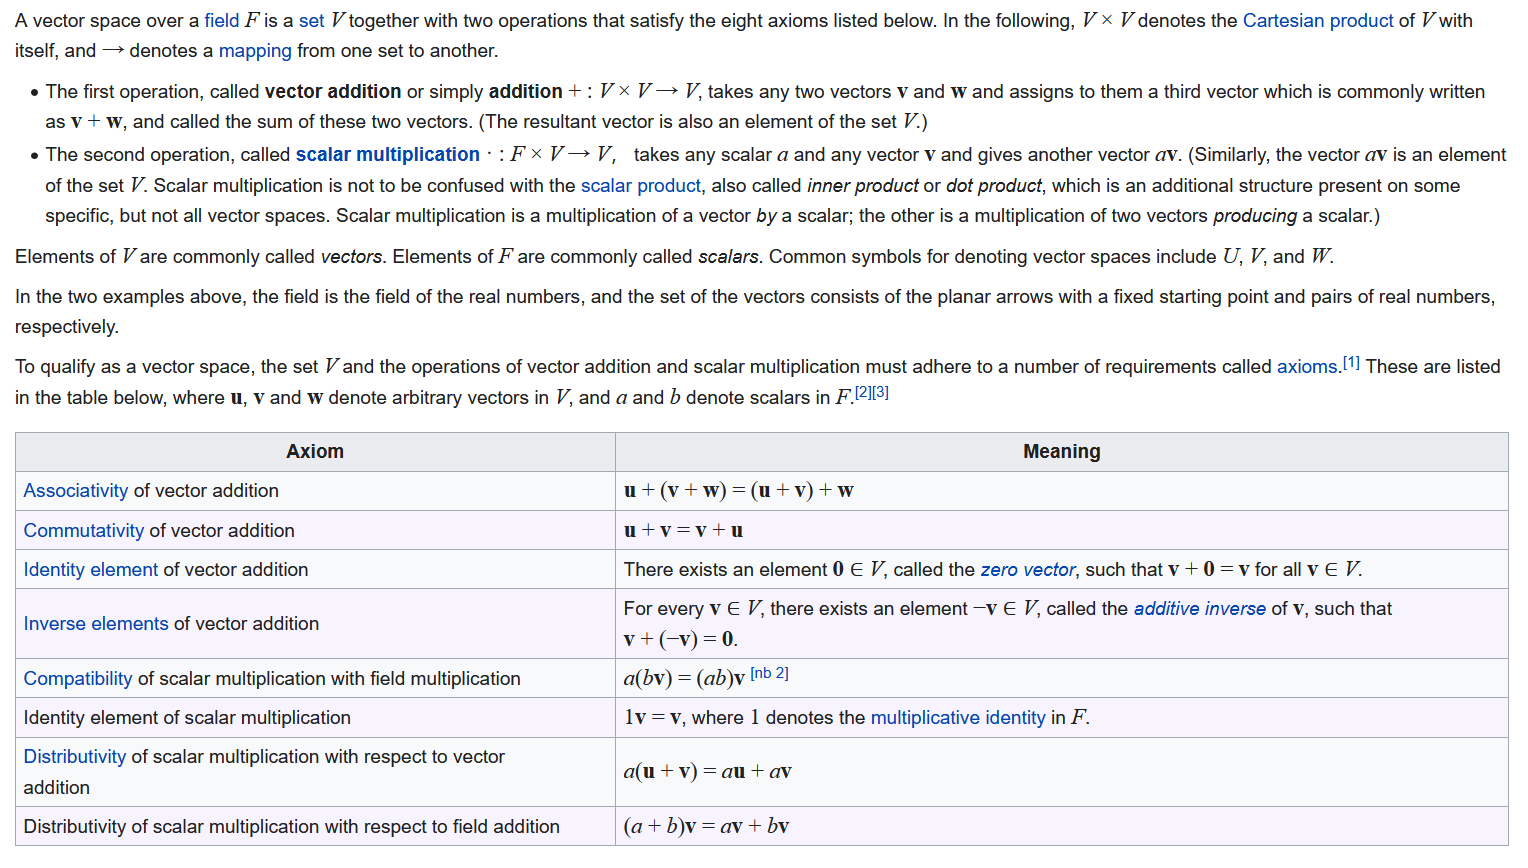
\includegraphics[width=1\linewidth,height=1\textheight]{images/vector-space-axioms-wikipedia_2} 

}

\caption{[Record scratch]  Yep, that's me, Vector Space, spewing a lot of incomprehensible stuff.  But I wasn't always like this.  Let me tell you a story...}\label{fig:unnamed-chunk-1}
\end{figure}

This reminds me of the joke about a cab driver driving around the Seattle area in a fog, and he asks a guy coming out of a building if he can tell the cabbie where he is. The guy looks at him and says, ``You're in a cab,'' and walks on. The cabbie says ``Perfect, I know where I am.'' The fare asks him how he can figure out anything from what the guy outside said, and the cabbie say, ``Well, he told me something that was completely true and completely useless. So this must be the Microsoft building.''

There's so many questions that should be triggered. Like:

\begin{itemize}
\tightlist
\item
  What are vectors, really?
\item
  What is a field, really?
\item
  What does it mean to add vectors?
\item
  What does it mean to multiply a vector by a scalar?
\item
  How do I know what other vector \(a \cdot \vec{u}\) becomes?
\item
  It looks like the scalar field talks about how \emph{scalar addition} and \emph{scalar multiplication} works. But vectors only talk about \emph{vector addition}. What's up with that?
\end{itemize}

The things I think about this are, \textbf{assuming I know the answer to the above questions}:

\begin{itemize}
\tightlist
\item
  Vectors work the way you think they should, it kinda-sorta works like addition for regular numbers.
\item
  Scalar multiplication works the way you think it should, it kinda-sorta works like addition and multiplication for regular numbers.
\item
  Scalars have both addition and multiplication, while vectors only have addition. That's gotta mean something.
\end{itemize}

  \bibliography{book.bib,packages.bib}

\end{document}
